\begin{frame}
  \frametitle{Características - Configuración de discos}
  \begin{itemize}
	  \item Configuración de discos IDE (\textit{Integrated Device Electronics}):
	  \begin{itemize}
	  	\item Master o Slave
	  	\item Primer y Segundo bus IDE
	  \end{itemize}
	  \item Denominación de los discos basada en los buses:
	  \begin{itemize}
	  	\item \textbf{/dev/hda}: configurado como Master en el 1º bus IDE
	  	\item \textbf{/dev/hdb}: configurado como Slave en el 1º bus IDE
	  	\item \textbf{/dev/hdc}: configurado como Master en el 2º bus IDE
	  	\item \textbf{/dev/hdd}: configurado como Slave en el 2º bus IDE
	  \end{itemize}
	  \item Particiones primarias $\rightarrow$ 1 a 4
	  \item Particiones logicas $\rightarrow$ desde 5 en adelante
  \end{itemize}
\end{frame}

\begin{frame}
  \frametitle{Características - Configuración de discos (cont.)}
  \begin{itemize}
	  \item Configuración de discos SCSI: se basa en \textit{LUN}
	  \item Denominación de los discos basada en la identificación de los buses:
	  \begin{itemize}
	  	\item \textbf{/dev/sda}
	  	\item \textbf{/dev/sdb}
	  	\item \textbf{/dev/sdc}
	  	\item \textbf{/dev/sdd}
	  	\item ...
	  \end{itemize}
	  \item La nomenclatura para los discos SATA es la misma
	  \item Particiones primarias:
	  \begin{itemize}
	  	\item Se numeran de la 1 a la 4 (solo estas se pueden marcar como activas $\rightarrow$ booteables)
	  \end{itemize}
	  \item Particiones extendidas:
	  \begin{itemize}
	  	\item Sus unidades o particiones lógicas se numeran a partir de la 5
	  \end{itemize}	  
  \end{itemize}
\end{frame}

\begin{frame}
  \frametitle{Características - Configuración de discos (cont.)}
  \begin{itemize}
	  \item Nueva nomenclatura utilizada:
	  \begin{itemize}
	  	\item Con la evolución de las distribuciones GNU/Linux, se comenzó a utilizar \textbf{``udev''} (\textit{.rules}) como gestor de dispositivos:
	  	\begin{itemize}
		  	\item Su función es controlar dinámicamente los archivos del /dev \textit{SOLO} en base al hardware detectado
		  	\item Soporta \textbf{Persistent Device Naming}
		  	\item Motiva su uso, el no poder garantizar que tras distintos arranques del SO, los dispositivos se sigan llamando de la misma manera. (Suponga disco 1 y 2, que disco 1 se quita y contorladoras SCSI/SATA mixtas)
		  	\item Reemplaza a \textit{devfs} y \textit{hotplug}
		  	\item Se desentiende del \textbf{Major} y \textbf{Minor Number}
		  	\item Se basa en eventos y permite que nuevos dispositivos sean agregados posteriormente al arranque
	  	\end{itemize}
	  \end{itemize}
  \end{itemize}
\end{frame}

\begin{frame}[fragile]
  \frametitle{Características - Configuración de discos (cont.)}
  \begin{itemize}
	  \item Desde Debian/Squeeze todos los dispositivos llamados hdX se denominan sdX 
	  \item Por estas y otras razones se adoptan 4 mecanismos nuevos para nomenclar\footnote{\url{http://wiki.debian.org/Part-UUID}}:
	  \begin{itemize}
	  	\item Nombres persistentes por \textbf{UUID} (\small{Universal Unique Identifier}):
	  	\begin{lstlisting}
$ ls –l /dev/disk/by-uuid/
2d781b26-0285-421a-b9d0-d4a0d3b55680 -> ../../sda1
31f8eb0d-612b-4805-835e-0e6d8b8c5591 -> ../../sda7
		\end{lstlisting}
		\item Utilizando \textbf{labels}
		\begin{lstlisting}
$ ls -l /dev/disk/by-label
data -> ../../sdb2
data2 -> ../../sda2
		\end{lstlisting}
	  \end{itemize}
  \end{itemize}
\end{frame}

\begin{frame}
  \frametitle{Soporte de instalación}
  \begin{itemize}
	  \item Existen diversos modos de instalar GNU/Linux:
	  \begin{itemize}
	  	\item Debemos tener en cuenta la arquitectura de hardware
	  	\begin{itemize}
		  	\item amd64: Arquitectura de 64 bits
		  	\item arm ó armel: Advanced Risc Machine
		  	\item i386: Arquitectura de 32 bits
		  	\item ia64: intelItanium o Intel Architecture-64
		  	\item Otras
	  	\end{itemize}
	  	\item Podemos instalarlo desde un CD descargao de la web
	  	\item Podemos instalarlo desde un USB: Unetbootin
	  	\begin{itemize}
	  		\item Permite crear instaladores o LiveCD utilizando USBs
	  	\end{itemize}
	  \end{itemize}
  \end{itemize}
\end{frame}

\begin{frame}
  \frametitle{Herramientas para particionar}
  \begin{itemize}
	  \item El particionado de un disco se lo puede realizar mediante:
	  \begin{itemize}
	  	\item Software destructivo: \textit{fdisk}
	  	\item Software no destructivo: \textit{fips}, \textit{gparted}
		\begin{figure}
		    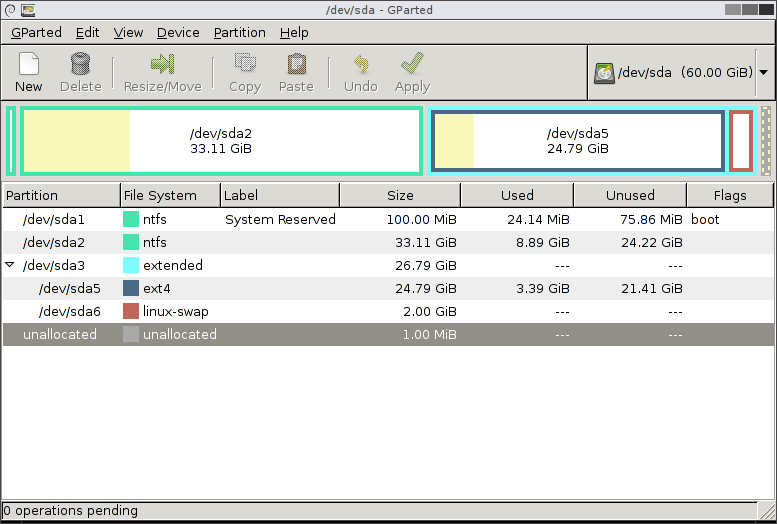
\includegraphics[scale=0.3]{images/gparted.png}
		\end{figure}
	  \end{itemize}
  \end{itemize}
\end{frame}

\begin{frame}
  \frametitle{Características}
  \begin{itemize}
	  \item No existe el concepto de \emph{extensión} en el nombre de un archivo
	  \item Los subdirectorios no se separan con el carácter `\textbackslash'
	  \item Es case sensitive
	  \item Entre un comando y sus parámetros debemos dejar obligatoriamente un espacio en blanco
	  \item Separación de entorno gráfico y texto
  \end{itemize}
\end{frame}

\begin{frame}
  \frametitle{Editor de textos \textbf{\emph{vim}}}
  \begin{itemize}
	  \item Presente en cualquier distribución de GNU/Linux
	  \item Posee 3 modos de ejecución:
	  \begin{itemize}
	  	\item Modo Insert (\textbf{Ins} o \textbf{i})
	  	\item Modo Visual (\textbf{v})
	  	\item Modo de Órdenes o Normal (\textbf{Esc})
	  \end{itemize}
	  \item Se le puede enviar una serie de comandos útiles
	  \begin{itemize}
	  	\item \textbf{w}: escribir cambios
	  	\item \textbf{q} ó \textbf{q!}: salir del editor
	  	\item \textbf{dd}: cortar
	  	\item \textbf{y}: copiar al portapapeles
	  	\item \textbf{p}: pegar desde el portapapeles
	  	\item \textbf{u}: deshacer
	  	\item \textbf{/}frase: busca ``frase'' dentro del archivo
	  \end{itemize}
  \end{itemize}
\end{frame}

\begin{frame}[fragile]
  \frametitle{Usuarios}
  \begin{itemize}
	  \item Todo usuario debe poseer credenciales para acceder al sistema
	  \begin{itemize}
	  	\item root: es el administrador del sistema (superusuario)
	  	\item otros: usuarios estándar del sistema (/etc/sudoers)
	  \end{itemize}
	  \item Archivos de configuración:
	  \begin{itemize}
	  	\item \textbf{/etc/passwd}
		\begin{lstlisting}
$ cat /etc/passwd
ndelrio:x:2375:500:Nico del Rio,,,,Usuarios:/home/admins/ndelrio:/bin/bash
		\end{lstlisting}	  	
	  	\item \textbf{/etc/group}
		\begin{lstlisting}
$ cat /etc/group		
infraestructura:x:500:
		\end{lstlisting}	  	
	  	\item \textbf{/etc/shadow}
		\begin{lstlisting}
$ cat /etc/shadow
ndelrio:$1$HamkgCYM$TtgfLJLplItxutaiqh/u9/:13273:0:99999:7:::
		\end{lstlisting}
	  \end{itemize}
  \end{itemize}
\end{frame}

\begin{frame}
  \frametitle{Usuarios (cont.)}
  \begin{itemize}
	  \item Comando para el manejo de usuarios:
	  \begin{itemize}
	  	\item \textbf{useradd} $<$nombreUsuario$>$:
	  	\begin{itemize}
	  		\item Agrega el usuario
	  		\item Modifica los archivos /etc/passwd
	  		\item Alternativa $\rightarrow$ \textbf{adduser}
	  	\end{itemize}
	  	\item \textbf{passwd} $<$nombreUsuario$>$:
	  	\begin{itemize}
	  		\item Asigna o cambia la contraseña del usuario
	  		\item Modifica el archivo /etc/shadow
	  	\end{itemize}
	  	\item \textbf{usermod} $<$nombreUsuario$>$:
	  	\begin{itemize}
	  		\item \textbf{-g}: modifica grupo de login (Modifica /etc/passwd)
	  		\item \textbf{-G}: modifica grupos adicionales (Modifica /etc/group)
	  		\item \textbf{-d}: modifica el directorio \emph{home} (Modifica /etc/passwd)
	  	\end{itemize}
	  	\item \textbf{userdel} $<$nombreUsuario$>$: elimina el usuario
	  	\item \textbf{groupdel} $<$nombreGrupo$>$: elimina el grupo
	  \end{itemize}
  \end{itemize}
\end{frame}

\begin{frame}[fragile]
  \frametitle{Permisos}
  \begin{itemize}
	  	\item Se aplican a directorios y archivos
	  	\item Existen 3 tipos de permisos y se basan en una notación octal:
	  	\begin{table}
		      \centering
		      \resizebox{10pc}{!}{
			  \begin{tabular}{| c | c | c |}
			      \hline
			      \bf Permiso & \bf Valor & \bf Octal \\
			      \hline
			      Lectura & R & 4 \\
			      \hline
			      Escritura & W & 2 \\
			      \hline
			      Ejecución & X & 1 \\
			      \hline
			  \end{tabular}
		      }
		\end{table}
		\item Se aplican sobre los usuarios:
		\begin{itemize}
			\item Usuario: permisos del dueño $\rightarrow$ \textbf{U}
			\item Usuario: permisos del grupo $\rightarrow$ \textbf{G}
			\item Usuario: permisos de otros usuario $\rightarrow$ \textbf{O}
		\end{itemize}
		\item Se utiliza el comando \textbf{chmod}:
		\begin{lstlisting}
$ chmod 755 /tmp/script
		\end{lstlisting}
  \end{itemize}
\end{frame}

\begin{frame}
  \frametitle{Entorno}
  \begin{itemize}
	  \item Algunos comandos útiles:
	  \begin{itemize}
	  	\item \textbf{ls}

	  	\item \textbf{cd}

	  	\item \textbf{mkdir}

	  	\item \textbf{rmdir}

	  	\item \textbf{rm}

	  	\item \textbf{mv}

	  	\item \textbf{cp}

	  	\item \textbf{man}
	  	
	  	\item \textbf{info}
	  \end{itemize}
  \end{itemize}
\end{frame}

\begin{frame}
  \frametitle{Bootloader}
  \begin{itemize}
  	\item El bootloader o cargador de arranque es un programa que permite cargar el Sistema Operativo. Puede llegar a cargar un entorno previo a la carga del sistema

  	\item Generalmente se utilizan los cargadores multietapas, en los que varios programas pequeños se van invocando hasta lograr la carga del SO

  	\item En cierto sentido, el código del \textit{BIOS/UEFI} forma parte del bootloader, pero el concepto está más orientado al código que reside en el \textit{Master Boot Record} (512b)

  	\item El MBR está formado por el \textit{MBC} (446b) y la \textit{Tabla de Particiones} (64b)

  	\item Sólo el MBC del Primary Master Disk es tenido en cuenta

  	\item El MBR existe en todos los discos, ya que contiene la tabla de particiones
  \end{itemize}
\end{frame}

\begin{frame}
  \frametitle{Proceso de arranque \textbf{System V}}
  \begin{enumerate}
	\item Se empieza a ejecutar el código del BIOS
	\item El BIOS ejecuta el POST
	\item El BIOS lee el sector de arranque (MBR)
	\item Se carga el gestor de arranque (MBC)
	\item El bootloader carga el \textit{kernel} y el \textit{initrd}
	\item Se monta el initrd como sistema de archivos raíz y se inicializan componentes esenciales (ej.: scheduler)
	\item El Kernel ejecuta el proceso \textit{init} y se desmonta el initrd
	\item Se lee el /etc/inittab
	\item Se ejecutan los scripts apuntados por el \textit{runlevel 1}
	\item El final del runlevel 1 le indica que vaya al runlevel por defecto
	\item Se ejecutan los scripts apuntados por el runlevel por defecto
	\item El sistema está listo para usarse
  \end{enumerate}
\end{frame}

\begin{frame}
  \frametitle{\textbf{init}}
  \begin{enumerate}
	\item Su función es cargar todos los subprocesos necesarios para el correcto funcionamiento del SO
	\item El proceso init posee el PID 1 y se encuentra en /sbin/init
	\item En SysV se lo configura a través del archivo /etc/inittab
	\item No tiene padre y es el padre de todos los procesos (\textit{pstree})
	\item Es el encargado de montar los filesystems y de hacer disponible los demás dispositivos
  \end{enumerate}
\end{frame}

\begin{frame}
  \frametitle{Runlevels}
  \begin{itemize}
	  	\item Es el modo en que arranca Linux (3 en \emph{Redhat}, 2 en \emph{Debian})

	  	\item El proceso de arranque lo dividimos en niveles

	  	\item Cada uno es responsable de levantar (iniciar) o bajar (parar) una serie de servicios
  \end{itemize}
\end{frame}

\begin{frame}[fragile]
  \frametitle{Runlevels}
  \begin{itemize}
	  	\item Se encuentran definidos en /etc/inittab
	  	\textcolor{orange}{id:nivelesEjecución:acción:proceso}
		\begin{itemize}
			\item \textbf{Id}: identifica la entrada en inittab (1 a 4 carácteres)
			\item \textbf{NivelesEjecución}: el/los niveles de ejecución en los que se realiza la acción
			\item \textbf{Acción}: describe la acción a realizar
			\begin{itemize}
				\item \textbf{wait}: inicia cuando entra al runlevel e init espera a que termine
				\item \textbf{initdefault}
				\item \textbf{ctrlaltdel}: se ejecutará cuando init reciba la señal \emph{SIGINT}
				\item \textbf{off}, \textbf{respawn}, \textbf{once}, \textbf{sysinit}, \textbf{boot}, \textbf{bootwait}, \textbf{powerwait}, etc.
			\end{itemize}
			\item \textbf{Proceso}: el proceso exacto que será ejecutado
		\end{itemize}
		\begin{lstlisting}
$ cat /etc/inittab
id:2:initdefault:
si::sysinit:/etc/init.d/rcS
ca::ctrlaltdel:/sbin/shutdown -t3 -r
		\end{lstlisting}
  \end{itemize}
\end{frame}

\begin{frame}
  \frametitle{Runlevels (cont.)}
  \begin{itemize}
	  	\item Existen 7, y permiten iniciar un conjunto de procesos al arranque o apagado del sistema
	  	\item Según el estándar:
	  	\begin{itemize}
	  		\item \textbf{0}: halt (parada)
	  		\item \textbf{1}: single user mode (monousuario)
	  		\item \textbf{2}: multiuser, without \textit{NFS} (modo multiusuario sin soperte de red)
	  		\item \textbf{3}: full multiuser mode console (modo multiusuario completo por consola)
	  		\item \textbf{4}: no se utiliza
	  		\item \textbf{5}: X11 (modo multiusuario completo con login gráfico basado en X)
	  		\item \textbf{6}: reboot
	  	\end{itemize}	  	
  \end{itemize}
\end{frame}

\begin{frame}[fragile]
  \frametitle{Runlevels (cont.)}
  \begin{itemize}
	  	\item Los scripts que se ejecutan están en /etc/init.d
	  	\item En /etc/rcX.d (donde X = 0..6) hay links a los archivos del /etc/init.d
	  	\item Formato de los links:

	  	\textcolor{orange}{[S\textbar K]$<$orden$>$$<$nombreScript$>$}
		\begin{lstlisting}
$ ls -1 /etc/rcS.d/
S55urandom
S70x11-common
		\end{lstlisting}
		\item \textbf{S}: lanza el script con el argument start
		\item \textbf{K}: lanza el script con el argument stop
  \end{itemize}
\end{frame}

\begin{frame}
  \frametitle{\textbf{insserv}}
  \begin{itemize}
	  	\item Se utiliza para administrar el orden de los enlaces simbólicos del /etc/rcX.d, resolviendo las dependencias de forma automática
	  	\item Utiliza cabeceras en los scripts del /etc/init.d que permiten especificar la relacion con otros scripts rc $\rightarrow$ LSBInit (Linux Standard Based Init)
		\item Es utilizado por \textit{update-rc.d} para instalar/remover los links simbólicos
  \end{itemize}
\end{frame}

\begin{frame}
  \frametitle{\textbf{insserv} (cont.)}
  \begin{itemize}
		\item Las dependencias se especifican mediante \textit{facilities} $\rightarrow$ \textbf{Provides} keyword
		\item Las facilities que comienzan con \$ se reservan para el sistema (\textit{\$syslog})
		\item Los scripts deben cumplir \textit{LSB init script}:
		\begin{itemize}
			\item Proveer al menos `start, stop, restart, force-reload and status'
			\item Retornar un código apropiado
			\item Declarar las dependencias
		\end{itemize}
  \end{itemize}
\end{frame}

\begin{frame}[fragile]
  \frametitle{\textbf{insserv} (cont.)}
  \begin{itemize}
	  	\item LSB init script headers:
		\begin{lstlisting}
### BEGIN INIT INFO
# Provides:          my_daemon
# Required-Start:    $syslog $remote_fs
# Required-Stop:     $syslog $remote_fs
# Default-Start:     2 3 4 5
# Default-Stop:      0 1 6
# Short-Description: This is a test daemon
# Description:       This is a test daemon
#                    This provides example about how to
#                    write a Init script.
### END INIT INFO
		\end{lstlisting}
  \end{itemize}
\end{frame}

\begin{frame}
  \frametitle{Proceso de arranque \textbf{Upstart}}
  \begin{itemize}
	  	\item Upstart fue el primer reemplazo propuesto para SystemV (\emph{Ubuntu}, \emph{Fedora, Debian}, etc.)
	  	\item Permite la ejecución de trabajos en forma asincrónica a través de eventos (\textit{event-based}) como principal diferencia con sysVinit que es estrictamente sincrónico (\textit{dependency-based})
	  	\item Estos trabajos se denominan \textbf{jobs}
		\item El principal objetivo de un job es definir servicios o tareas a ser ejecutadas por init
		\item Son scripts de texto plano que definene las acciones/tareas (unidad de trabajo) a ejecutar ante determinados eventos		
	  	\item Cada job es definido en el /etc/init (\textbf{.conf})
	  	\item Suelen ser de dos tipos:
	  	\begin{itemize}
	  		\item \textbf{Task}: ejecución finita (\textit{task}) $\rightarrow$ not respawning $\rightarrow$ exit 0 o uso de \textit{stop}
	  		\item \textbf{Service}: ejecución indeterminada $\rightarrow$ respawning
	  	\end{itemize}	  	
  \end{itemize}
\end{frame}

\begin{frame}
  \frametitle{Proceso de arranque \textbf{Upstart} (cont.)}
  \begin{itemize}
	  	\item Los jobs son ejecutados ante eventos (arranque del equipo, inserción de un dispositivo USB, etc.):
	  	\begin{itemize}
	  		\item Es posible crear eventos pero existen algunos de manera estándar\footnote{\url{http://people.canonical.com/~jhunt/upstart/upstart-states.png}}
	  		\item Definido por \textbf{start on} y \textbf{stop on}
	  	\end{itemize}  
  		\item Es compatible con SystemV $\rightarrow$ /etc/init/rc-sysinit.conf, runlevels, scripts en /etc/init.d, objetivo start y stop
	  	\item Cada job posee un objetivo (\textit{goal start/stop}) y un estado (\textit{state})
	  	\begin{itemize}
	  		\item En base a ellos se ejecuta un proceso específico
	  		\item Al inicio, init emite el evento \textit{startup}
	  	\end{itemize}
  \end{itemize}
\end{frame}

\begin{frame}
  	\frametitle{Proceso de arranque \textbf{Upstart} (cont.)}
  	\begin{itemize}
		\item Un job puede tener uno o varias tareas ejecutables como parte de su ciclo de vida y siempre debe existir la tarea principal
	  	\item Las tareas de un job se definen mediante \textit{exec} o \textit{script ... end script}
	  	\item A través de \textit{initctl} podemos administrar los jobs del demonio de Upstart:
	  	\begin{itemize}
	  		\item start $<$job$>$: cambia el objetivo a start del job especificado
	  		\item stop $<$job$>$: cambia el objetivo a stop del job especificado
	  		\item emit $<$event$>$: event es emitido causando que otros jobs cambien a objetivo start o stop
	  	\end{itemize}
	  	\item No más /etc/inittab
  	\end{itemize}
\end{frame}

\begin{frame}
  	\frametitle{\textbf{Systemd}}
  	\begin{itemize}
		\item Es un sistema que centraliza la administración de demonios y librerias del sistema
		\item Mejora el paralelismo de booteo
		\item Puede ser controlado por \textbf{systemctl}
		\item Compatible con SysV $\rightarrow$ si es llamado como \emph{init}
		\item El demonio \emph{systemd} reemplaza al proceso init $\rightarrow$ este pasa a terner \emph{PID 1}
		\item Los runlevels son reemplazados por \textbf{targets}
		\item Al igual que con Upstart el archivo /etc/inittab no existe más
  	\end{itemize}
\end{frame}

\begin{frame}
  	\frametitle{\textbf{Systemd} (cont.)}
  	\begin{itemize}
		\item Las unidades de trabajo son denominadas \textbf{units} de tipo:
		\begin{itemize}
			\item \textbf{Service}: controla un servicio particular (\emph{.service})
			\item \textbf{Socket}: encapsula IPC, un sockect del sistema o file system \emph{FIFO} (\emph{.socket}) $\rightarrow$ sockect-based activation
			\item \textbf{Target}: agrupa units o establece puntos de sincronización durante el booteo (\emph{.target}) $\rightarrow$ dependencia de unidades
			\item \textbf{Snapshot}: almacena el estado de un conjunto de unidades que puede ser restablecido más tarde (\emph{.snapshot})
			\item etc.
		\end{itemize}
		\item Las units pueden tener dos estados $\rightarrow$ \textbf{active} o \textbf{inactive}
  	\end{itemize}
\end{frame}

\begin{frame}
  \frametitle{\textbf{Systemd} (cont.)}
  \begin{figure}
	    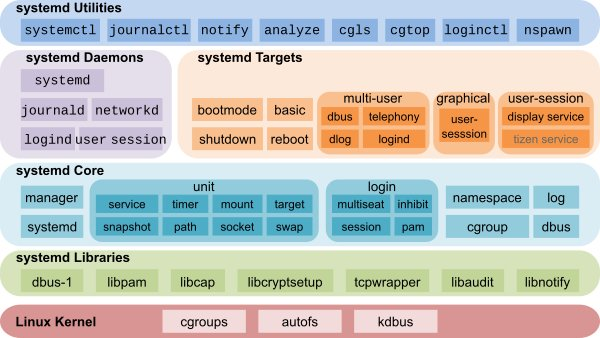
\includegraphics[scale=0.5]{images/systemd.jpg}
  \end{figure}
\end{frame}

\begin{frame}
  	\frametitle{\textbf{Systemd} - Activación por Socket}
  	\begin{itemize}
		\item No todos los servicios que se inician en el booteo se utilizan:
		\begin{itemize}
			\item impresora
			\item servidor en el puerto 80
			\item etc.
		\end{itemize}
		\item Es un mecanismo de iniciación bajo demanda $\rightarrow$ podemos ofrecer una variedad de servicios sin que realmente esten iniciados
		\item Cuando el sockect recibe una conxión spawnea el servicio y le pasa el socket
		\item No hay necesidad de definir dependencias entre servicios $\rightarrow$ se inician todos los sockects en primer medida
  	\end{itemize}
\end{frame}

\begin{frame}
  	\frametitle{\textbf{Systemd} - \textbf{cgroups}}
  	\begin{itemize}
		\item Permite organizar un grupo de procesos en forma jerárquica
		\item Agrupa conjunto de procesos relacionados (por ejemplo, un servidor web Apache con sus dependientes)
		\item Tareas que realiza:
		\begin{itemize}
			\item Tracking mediante subsistema cgroups $\rightarrow$ no se utiliza el PID $\rightarrow$ doble \emph{fork} no funciona para escapar de systemd
			\item Limitar el uso de recursos
			\item etc.
		\end{itemize}
  	\end{itemize}
\end{frame}

\begin{frame}[fragile]
  	\frametitle{\textbf{fstab}}
  	\begin{itemize}
		\item Define qué particiones se montan al arranque
		\item Su configuración se encuentra en /etc/fstab:
		\begin{lstlisting}
$ cat /etc/fstab
# <file system> <mount point> <type> <options> <dump> <pass>
/dev/sda1 / ext4 errors=remount-ro 0       1

UUID=3FDE00F9523092AE /home/iso/datos ntfs user,auto,rw,exec,uid=1000,gid=1000,umask=000 0 2

/dev/sda2 none swap sw 0 0
		\end{lstlisting}
		\item Opciones:
		\begin{itemize}
			\item \textbf{user}: cualquier usuario puede montar la partición
			\item \textbf{auto}: monta la partición al inicio
			\item \textbf{ro}: read only, \textbf{rw}: read and write
			\item etc.
		\end{itemize}
  	\end{itemize}
\end{frame}

\begin{frame}
  	\frametitle{Redirecciones}
  	\begin{itemize}
		\item Al utilizar redirecciones mediante \textbf{$>$} (destructiva):
		\begin{itemize}
			\item Si el archivo de destino no existe, se lo crea
			\item Si el archivo existe, se lo trunca y se escribe el nuevo contenido
		\end{itemize}
		\item Al utilizar redirecciones mediante \textbf{$>>$} (no destructiva):
		\begin{itemize}
			\item Si el archivo de destino no existe, se lo crea
			\item Si el archivo existe, se agrega la información al final
		\end{itemize}
  	\end{itemize}
\end{frame}

\begin{frame}[fragile]
  	\frametitle{Uso de \textbf{\textbar}}
  	\begin{itemize}
		\item El ``\textbar'' nos permite comunicar dos procesos 
		por medio de unpipe o tubería desde la \emph{shell}
		\item El pipe conecta \textit{stdout} (salida estándar) del primer comando con la \textit{stdin} (entrada estándar) del segundo.
		\item Por ejemplo:	
		\begin{lstlisting}
$ ls | more
		\end{lstlisting}
		\begin{itemize}			
			\item Se ejecuta el comando \emph{ls} y la salida del mismo, es enviada como entrada del comanda \emph{more}
		\end{itemize}
		\item Se pueden anidar tantos pipes como se deseen
		\item ¿Cómo haríamos si quisiéramos contar la cantidad de usuarios del sistema que en su nombre de usuario aparece una letra ``a''?
		\pause
		\begin{lstlisting}
$ cat /etc/passwd | cut -d: -f1 | grep a | wc -l
		\end{lstlisting}
  	\end{itemize}
\end{frame}
